\documentclass[12pt,a4paper,titlepage]{report}

\usepackage[utf8x]{inputenc}
\usepackage{ucs}
\usepackage[english]{babel}
\usepackage{caption}
\usepackage{xspace}% For a variable space after a macro.
\usepackage{amsmath}
\usepackage[round]{natbib}
\usepackage{amsfonts}
\usepackage{amssymb}
\usepackage{wrapfig}
\usepackage[textsize=tiny]{todonotes}
\usepackage{graphicx}
\usepackage[left=2cm,right=2cm,top=2cm,bottom=2cm]{geometry}

\bibliographystyle{plainnat}

\author{A.J. Bonnema}
\title{Architecture document}
\begin{document}

\newcommand{\w}[1]{\textsc{#1}}%
\newcommand{\Noc}{\textsc{NoC}\xspace}% 
\newcommand{\xmas}{\textsc{XMas}\xspace}%
\newcommand{\fltk}{\textsc{fltk}\xspace}%
\newcommand{\boost}{\textsc{Boost}\xspace}%
\newcommand{\opengl}{\textsc{OpenGL}\xspace}%
\newcommand{\qt}{\textsc{Qt}\xspace}%
%\newcommand{\code}[1]{\verb%#1%}%
\newcommand{\code}[1]{\texttt{#1}}%
\newcommand{\qobj}{\code{Q\_OBJECT}}%

\chapter{Introduction}

\paragraph{Document use} The document is meant for
developers new to this project and for maintainers
considering a change. It allows a high level view 
and drilling down some to isolate the 
partition that needs change. Finally, the document
is for programmers looking for design guidelines.

\paragraph{Document structure} The document consists
of the high level class diagrams, some sequence diagrams,
some design patterns and finally the design guidelines and 
specific platform dependencies.

\paragraph{Document maintenance} Some of the diagrams -- especially 
the introductory architectural drawings -- were created with \w{Dia}\footnote{you 
can find \w{Dia} at http://sourceforge.net/projects/dia-installer/}.

Most of the \w{UML} diagrams we created with \w{Umbrello}. Be careful to use the most 
recent version as possible. From the the menu option \w{export all diagrams as
picture} or the equivalent option for one diagram one can create an image for
this document.

\paragraph{Naming} Make sure to create names without spaces so the exported filenames
will also be valid. Even though most OS's can work around spaces they
still are a pain in the neck.



cite\chapter{Architecture Overview}

This document partitions the system into 3 parts:

\begin{description}
	\item[Design Tool] This is the graphical and textual representation of the
	\Noc.
	\item[VT Plugin tool] This is the connection between the design tool and the verification
	tools. 
	\item[VT] The specific verification tools. This currently includes the combinatoric cycle 
	checker, the deadlock checker and may include tools. They all fit into and use the VT plugin
	tool.
\end{description}

This document describes the design tool and the VT plugin. Each verification tool has its own papers
and documentation. As far as necessary for the plugin, requirements from the VTs are included.

\todo[inline]{Consider a how-to-guide for creating a plugin.}

\section{Partitioning}

\begin{center}
	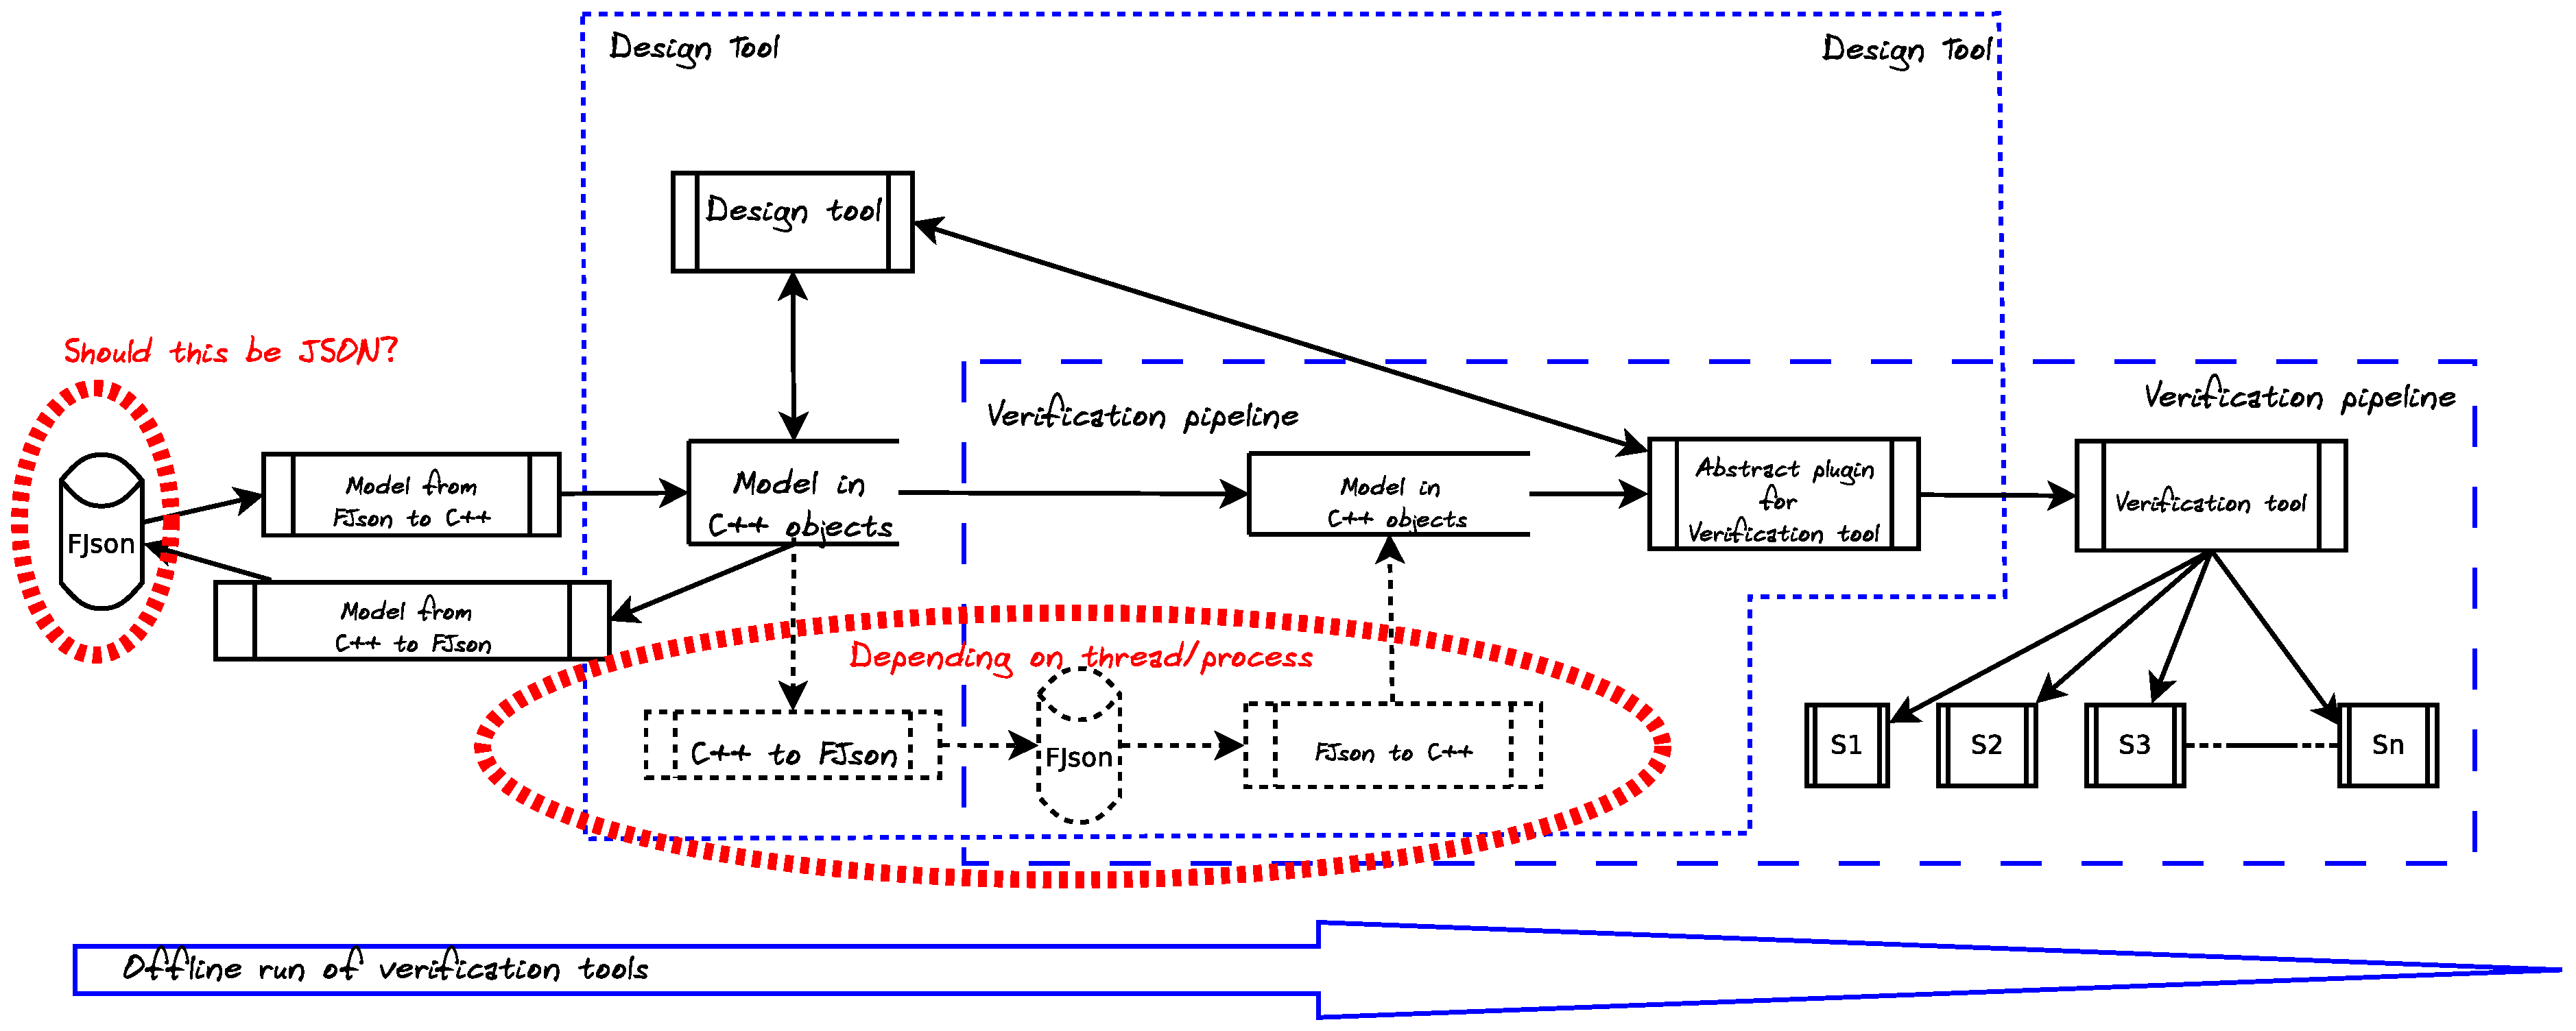
\includegraphics[width=.9\linewidth]{../architecture-tool-scope}
\end{center}

The complete tool consists of a graphical design tool and a verification pipeline.
The design tool runs online (in a graphical environment) and is meant to aid in 
designing a Network on Chip (\Noc). The verification tools can run in the online 
(graphical) environment or in an offline (commandline) environment and are meant 
to do consistency and correctness checks on a model.
The case of offline verification is useful for verifying a model that is 
too big to verify completely during graphical edit cycles.

\paragraph{Usage goal} The goals for running the graphical editor 
or the verification pipeline may either be creating an \Noc or 
testing a verification tool. In both cases the dynamics are the same.

\paragraph{Plugin architecture} The verification tools and the graphical 
design toolkit communicatie through a plugin architecture.
The runtimes for verification tools will vary -- depending on the input --
from several seconds to a few minutes or longer. For that reason the 
verification tools run relatively independently from the graphical 
design toolkit. 

\todo[inline]{How will the plugin architecture overlap between 
the online and the offline versions of running the verification tools? I.e. how
will this architecture reflect on the currently existing verification tools?}


We will flatten the model on behalf of the verification tools in the VT plugin.
Currently verification tools cannot work with composites but are planned for the future 
(see \citep[question 14 on page 32]{ou:team23-endreport}).

\section{Graphical Design Tool Dynamics}

\pagedepth\maxdimen

\begin{wrapfigure}[9]{i}{0.3\linewidth}
	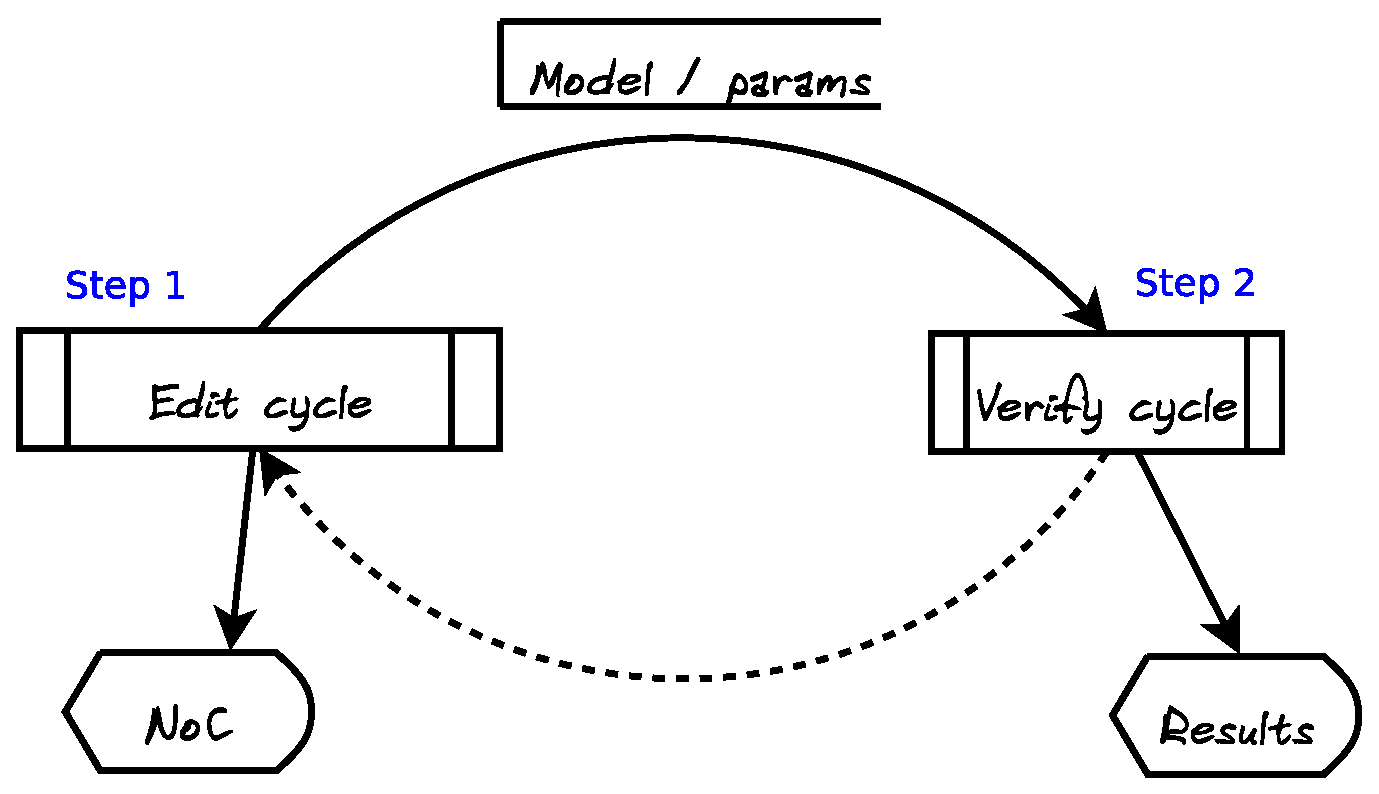
\includegraphics[width=.95\linewidth]{../architecture-dynamic-overview}
	\caption{Dynamic process in overview}
	\label{fig:overview-dynamic}
\end{wrapfigure}

The graphical editor of \Noc consists of a toolkit containing
the \xmas primitives, the composites available in separate 
libraries, the graphical window, and the commands to 
prepare and execute the verification tools. The process of 
designing an \Noc consists of alternating an edit cycle with a verify cycle 
(see figure \ref{fig:overview-dynamic}).

\paragraph{Step 1 Edit cycle} The editor adds components (primitives or 
composites) to the \Noc diagram filling in their parameters and connecting 
components as necessary. Once satisfied the editor switches to prepare 
for the verfication cycle.

\paragraph{Step 2 Verification cycle} 
Firstly, the editor chooses the verification tools to be run.
Secondly, the editor fills in the relevant parameters for running the selected 
verification tools. Finally, the editor starts the verification processes causing
the controller to copy the parameters and the current \Noc model and start
the verification tools selected. See figure \ref{fig:dynamic-arch} for a 
detailed illustration.

\begin{center}
	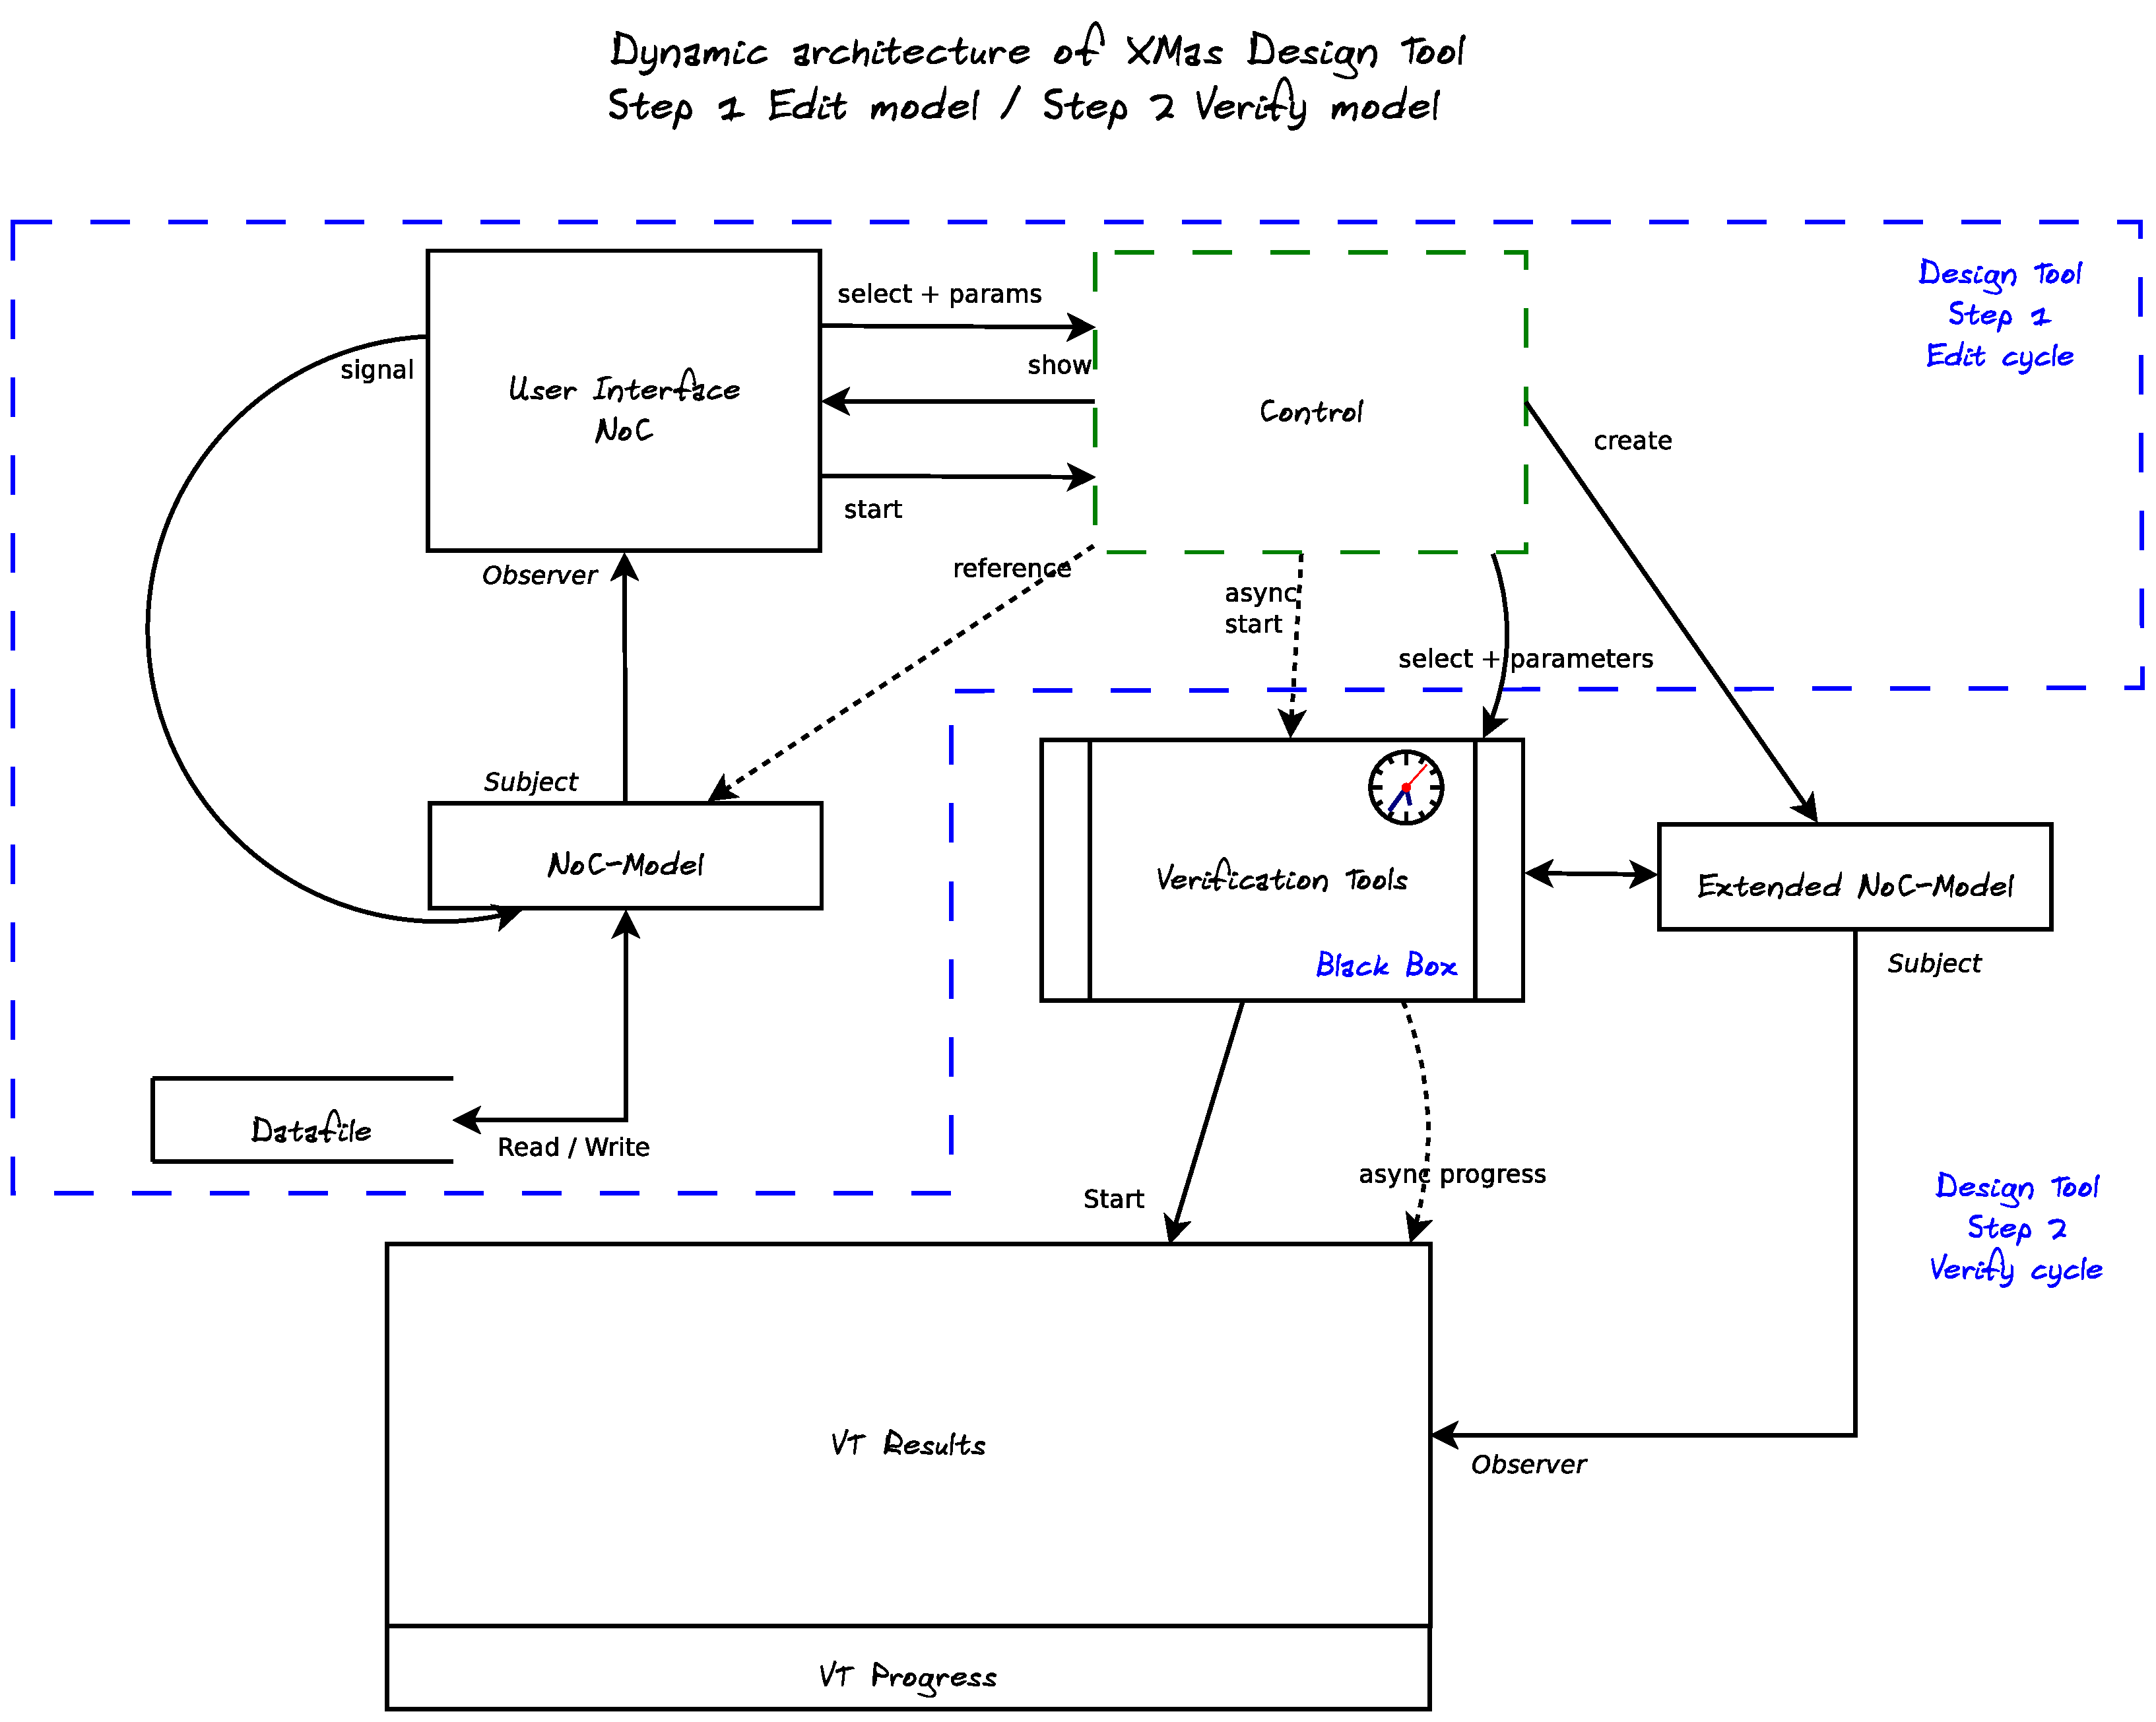
\includegraphics[width=.95\linewidth]{../architecture-dynamic}
	\captionof{figure}{Dynamic process of editing and verifying}
	\label{fig:dynamic-arch}
\end{center}

\paragraph{Verification results} The verification tools 
will show their results and their progress while running. 
Depending on the verification tool, the results could be
graphical or textual or both. The plugin will show either
textual or graphical output allowing for addition textual 
or graphical markings on the network drawing.

Remark that the verification tools run in their own
thread or process depending on whether the output will be
shown in the design UI thread or an independent 
UI thread\todo{TBD}.

\paragraph{Communication pattern} The user interface implements
the observer pattern with respect to data changes.
Both the design tool and the verification plugin use this pattern to
propagate changes in the model to the user interface.

\section{Verification pipeline}

\paragraph{Scope.} The verification pipeline itself is
not in scope for the graphical editor. The connection to the verification 
pipeline is through the plugin architecture, where a plugin is wrapped 
in a C++ class that derives from \w{VerificationTool}.


\section{Verification Tool repository}

\paragraph{Tool repository} The design tool needs a reference to each 
verification tool in order to have the user select the 
verification tools to run. This information whether stored
in the code or stored in a file, we call the tool repository.
Each tool needs an entry in the tool repository.

\paragraph{Tool meta information} Each tool needs certain parameters 
filled in. The tool should provide a method of entering this data 
both through a graphical user interface and through providing a 
file with input.

\paragraph{Generic meta information} Some parameters directly influence 
the structure of the component. An example is a number $n$ that
specifies the number of primitives in a spidergon topology (see \cite{chatterjee-kishinevsky:xmas}\todo{check}).
\todo[inline]{These parameters need special care when passing through to the
verification tools. whether and how to flatten is still subject to discussion.}

\paragraph{Control in a loosely coupled way} An way to implement 
the verification repository is to have each verification tool register 
with a controller. The registration involves informing the controller
about function, and parameters of the specific verification tool. 
The graphical editor will ask the controller for available 
verification tools. The verification tools should also provide
a dialog for entering the parameters. This way the connection between 
the graphical design tool and the verification pipeline is as loose 
as possible while keeping control over the dynamics in the process.


\section{Component repository}

\todo[inline]{We need a (non-programmatic) way of defining new components, whether 
primitive or composite.}

\section{Model repository}

\todo[inline]{Some way of storing models.}
\chapter{Architecture Design Guidelines}

\section{Leading requirements}

The following list of leading requirements is meant to guide the creation and maintenance
of design guidelines and design decisions. The most important requirements are first
and foremost leading arguments in any comparison of alternatives. 

\begin{description}

	\item[Portability leads] We need the design tool to run equally well on all defined platforms
	and possibly platforms not (yet) defined. For that reason portability is a leading requirement.
	
	\item[Ease of use seconds] We need the design tool to assist in the design of \Noc and
	the development of verification tools with respect to \Noc designs. For that reason the design
	tool should facilitate these activities as much as possible. 
	
	\item[Maintainability third] The ease of maintenance was one of the primary requirements and
	as such should guide future design decisions. 
	
	\item[Performance follows] Under normal circumstances performance arguments should not lead.
	However, unacceptable performance will override all other considerations, because
	unacceptable performance disrupts use of the tool. 
	
	\item[Remark] What is acceptable performance is subjective. 
	
\end{description}

\paragraph{Example} When given a choice between alternatives with equal portability and 
ease of use consequences, the maintenance arguments should lead at the cost of performance 
provided the performance seems acceptable.

\section{High level design guidelines}

\begin{description}

	\item[C++ constructs lead] We strive to use C++ of the latest standard, currently C++ 2011.
	This implies the use of the C++ library including containers.
	
	\item[Boost] We use \boost as our goto library for portability. For mechanisms that would
	otherwise require platform dependent code we use \boost. Messaging, process control and
	interprocess communication is all directed through \boost.
	
	\item[fltk] We use the GUI library \fltk (pronounce ``\texttt{fulltick}'') for all GUI code.
	This takes care of most of the performance concerns for a graphical user interface.
	
	\item[OpenGL] Where we need extra drawing power we use \opengl or the \fltk \w{gl} extentions.
	This takes care of the remaining performance concerns that might exist.
	
\end{description}

\section{Observer pattern}

We use our own observer pattern as described in the \w{GoF}. 
Figure \ref{fig:observer-applied} the pattern applies the principle. 
Any object wanting to observe one of the subjects, needs to 
derive from \w{ConcreteObserver}.

\begin{center}
	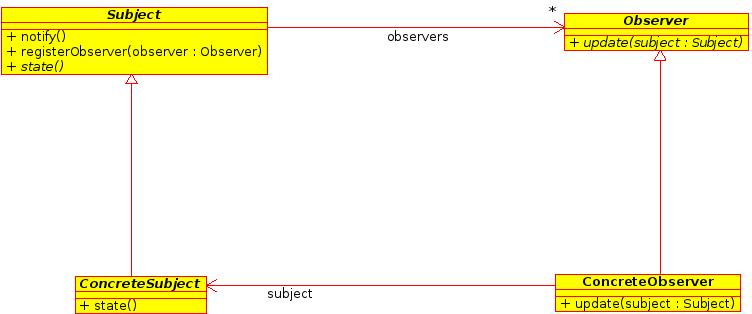
\includegraphics[width=.7\linewidth]{ObserverClassDiagram.jpeg}
	\captionof{figure}{Observer pattern as described in \w{GoF}}
	\label{fig:observer-pattern}
\end{center}

\begin{center}
	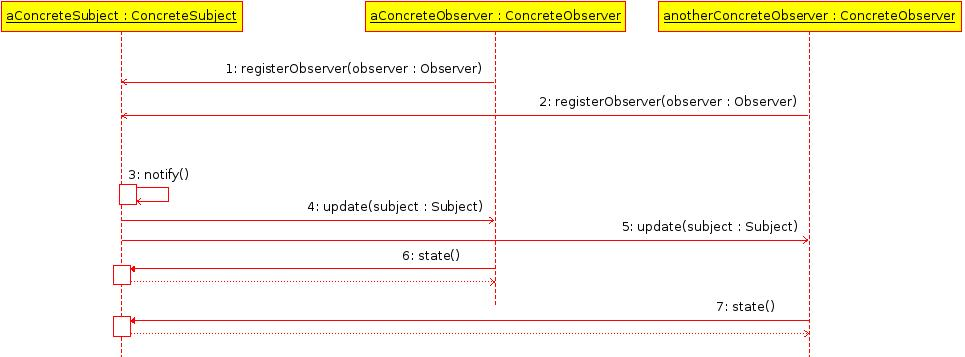
\includegraphics[width=.7\linewidth]{ObserverSequenceDiagram.jpeg}
	\captionof{figure}{Observer pattern applied}
	\label{fig:observer-applied}
\end{center}


\section{Architecture High Level Diagrams}

%\begin{center}
%	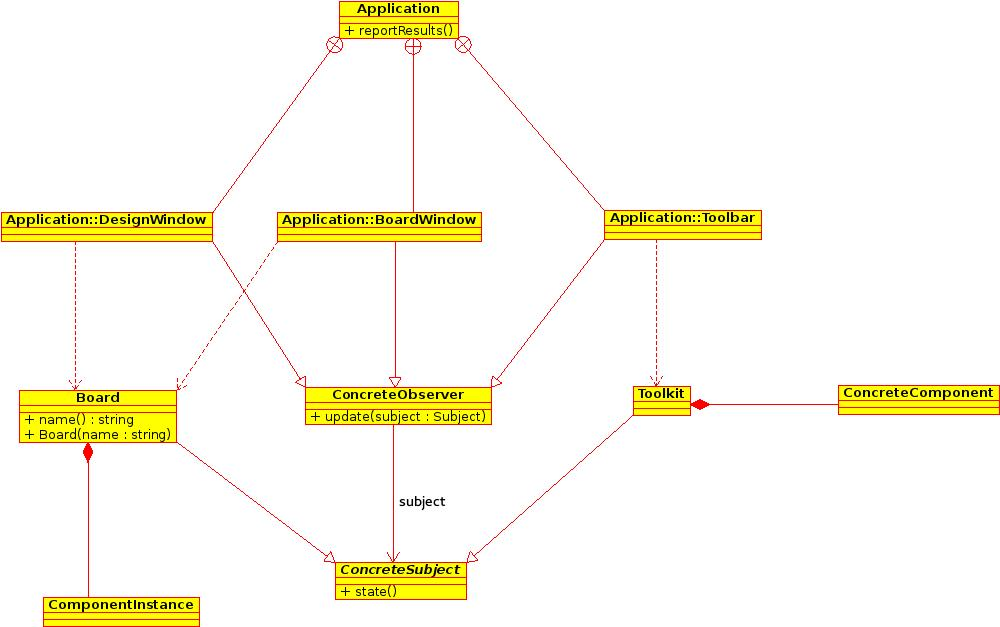
\includegraphics[width=.9\linewidth]{UI_ClassDiagramMain.jpeg}
%	\captionof{figure}{User Interface high level class diagram}
%	\label{fig:ui_class_diagram}
%\end{center}

\todo[inline]{To do}

\section{Plugin construction}

Any verification tool must override the \w{ConcreteVerificationTool} 
and register with the application in order to have the option
of being executed on request. 

\begin{center}
	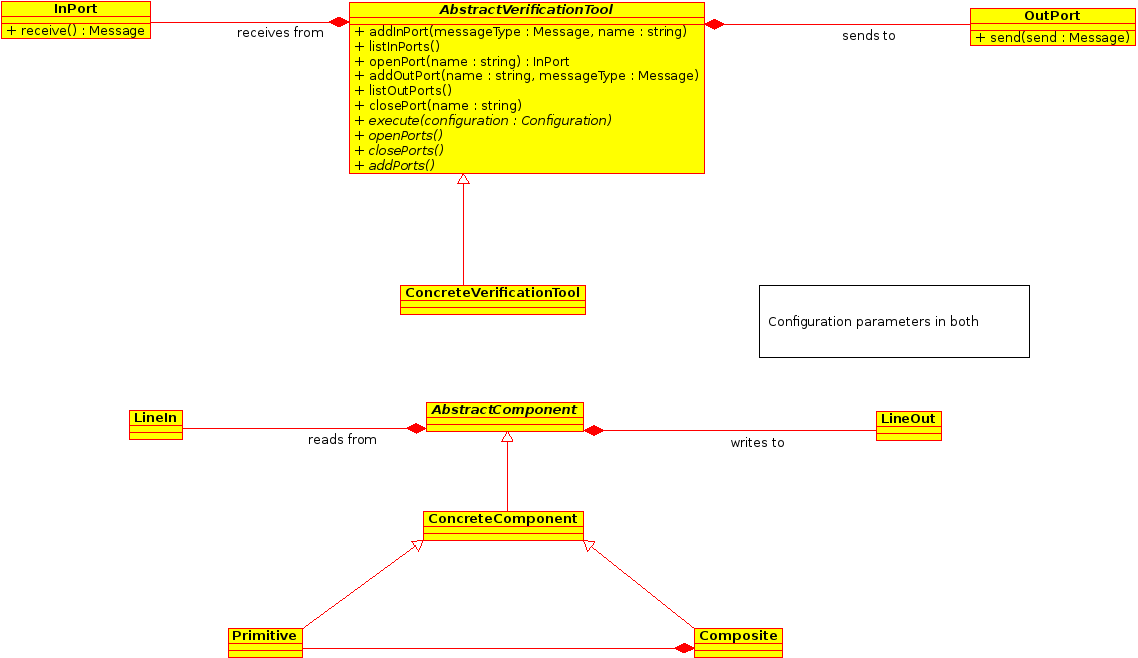
\includegraphics[width=.9\linewidth]{PluginClassDiagram}
	\captionof{figure}{The plugin to build verification tools.}
	\label{fig:plugin-class-diagram}
\end{center}


\section{Language guidelines}

\subsection{C++ construct preferences}

Our coding strives to use the best of C++ 2011 and to
avoid coding that may be error prone. Sometimes a construct like

\begin{verbatim}using typename = std::vector<std::string>\end{verbatim}

\noindent should enhance readability provided the \verb%typename% chosen
makes sense in the context. Table \ref{tab:coding-preferences} lists the
current coding preferences.

\begin{center}
	\begin{tabular}{|p{10em}|p{10em}|p{10em}|}
	\hline
	{\bf Prefer} & {\bf Avoid} & {\bf Comment}\\\hline
	shared\_ptr, unique\_ptr & pointer & \\
	weak\_ptr & & with specific reason\\
	make\_shared() & new, delete & \\ 
	\hline
	\end{tabular}
	\captionof{table}{Preferences in coding guidelines}
	\label{tab:coding-preferences}
\end{center}

\paragraph{Memory management}
Using smart pointers avoids many of the pointer pitfalls causing
memory leaks to occur that might go undetected. When creating
dynamic memory preferring \verb%make_ptr% leads to code that 
avoids mixing the old paradigm (\verb%new% and \verb%delete%) with
the new. 

\paragraph{weak\_ptr} 
A \verb%weak_ptr% we use only with a 
specific motivation because it requires extra work to make sure 
that we are referencing an existing smart pointer i.e. it has 
not been deleted yet.

\paragraph{allocator}
In most situations the library versions of \verb%vector%, 
\verb%list% and \verb%string% should suffice and be performant
enough for our goals. In case explicit memory management is 
necessary we could use the library class \verb%allocator%. This
ensures efficient allocation and deallocation of memory with
knowledge of type information and separating allocation and
construction of memory.

\chapter{Platform dependent constraints}

\section{Home of the software}

\section{Linux}

\subsection{Download and install}

\subsection{Regular build procedure}

\section{Macintosh}

\subsection{Download and install}

\subsection{Regular build procedure}

\subsection{Build limitations}

\section{MS Windows}

\subsection{Download and install}

\subsection{Regular build procedure}


\appendix
\bibliography{references}
\end{document}
